\documentclass[conference]{IEEEtran}
\IEEEoverridecommandlockouts
% The preceding line is only needed to identify funding in the first footnote. If that is unneeded, please comment it out.
%Template version as of 6/27/2024

\usepackage{cite}
\usepackage{amsmath,amssymb,amsfonts}
\usepackage{algorithmic}
\usepackage{graphicx}
\usepackage{textcomp}
\usepackage{xcolor}
\def\BibTeX{{\rm B\kern-.05em{\sc i\kern-.025em b}\kern-.08em
    T\kern-.1667em\lower.7ex\hbox{E}\kern-.125emX}}
\begin{document}

\title{The YOLO Model for Web Segmentation: Re-Evaluation and Advancements
}

\author{\IEEEauthorblockN{1\textsuperscript{st} Given Name Surname}
\IEEEauthorblockA{\textit{dept. name of organization (of Aff.)} \\
\textit{name of organization (of Aff.)}\\
City, Country \\
email address or ORCID}
\and
\IEEEauthorblockN{2\textsuperscript{nd} Given Name Surname}
\IEEEauthorblockA{\textit{dept. name of organization (of Aff.)} \\
\textit{name of organization (of Aff.)}\\
City, Country \\
email address or ORCID}
\and
\IEEEauthorblockN{3\textsuperscript{rd} Given Name Surname}
\IEEEauthorblockA{\textit{dept. name of organization (of Aff.)} \\
\textit{name of organization (of Aff.)}\\
City, Country \\
email address or ORCID}
\and
\IEEEauthorblockN{4\textsuperscript{th} Given Name Surname}
\IEEEauthorblockA{\textit{dept. name of organization (of Aff.)} \\
\textit{name of organization (of Aff.)}\\
City, Country \\
email address or ORCID}
\and
\IEEEauthorblockN{5\textsuperscript{th} Given Name Surname}
\IEEEauthorblockA{\textit{dept. name of organization (of Aff.)} \\
\textit{name of organization (of Aff.)}\\
City, Country \\
email address or ORCID}
\and
\IEEEauthorblockN{6\textsuperscript{th} Given Name Surname}
\IEEEauthorblockA{\textit{dept. name of organization (of Aff.)} \\
\textit{name of organization (of Aff.)}\\
City, Country \\
email address or ORCID}
}

\maketitle

\begin{abstract}

Web page segmentation, the partitioning of a webpage into meaningful blocks, is crucial for various web applications like accessibility evaluation and information extraction. While early methods relied on DOM tree analysis, they often fail to capture the user's visual perception of web content, particularly with modern web technologies. This paper focuses on purely visual web segmentation using the YOLO (You Only Look Once) series. We investigate YOLOv5 and its web segmentation variant, YOLO-WS, previously benchmarked on the visually-labeled Webis-Webseg-20 dataset. We reimplement YOLO-WS, revisit its benchmark performance, and evaluate the latest YOLOv11 architecture against both YOLOv5 and our reimplemented YOLO-WS. Finally, we explore the impact of input resolution on segmentation accuracy for website screenshots.\\

\end{abstract}

\begin{IEEEkeywords}
visual webpage segmentation, deep learning for web layout analysis, YOLO-based web content detection
\end{IEEEkeywords}

\section{Introduction}
Web segmentation is the task of dividing a web page into meaningful blocks, which is important in applications such as accessibility evaluation, information extraction and web automation. Early web segmentation methods relied heavily on DOM-tree analysis \cite{VIPS, DOM-structure, HEPS}, but faced limitations as DOM structures often fail to represent visual content accurately, especially with modern web development practices using complex CSS and JavaScript transformations.

Recent research increasingly focuses on visual web segmentation, processing the rendered visual representation of web pages directly. While mixed DOM-based models attempt to bridge the gap by combining structural and visual information, the de facto standard dataset for evaluating web segmentation performance is the purely visually labeled dataset Webis-Webseg-20 \cite{kiesel:2020b}. Therefore, this paper focuses on purely visual-based web segmentation methods.

Building upon the promising performance of the YOLO (You Only Look Once) series in visual object detection, this work explores the application of YOLOv5 and its web-segmentation version YOLO-WS proposed by \cite{YOLO-WS} which was benchmarked on Webis-Webseg-20. YOLOv5 is a proprietary model from Ultralytics (unpublished) \cite{yolov5}. However, it is licensed under the AGPL-3.0, making it accessible and modifiable for educational purposes. We seek to reimplement YOLO-WS and revisit benchmarking on Webis-Webseg-20. Additionally, we evaluate the latest YOLOv11 model against YOLOv5 and YOLO-WS, and we hypothesize that increasing input sizes from 512x512 and preserving the images aspect ration could improve performance for website screenshots.

\section{Data \& Experiments}

\subsection{Data}

The Webis-Webseg-20 dataset contains 42'450 manually annotated webpage segmentation samples from 8'490 webpages. Human annotators used a visual annotator interface where annotators could draw segments on a screenshot of the webpage. The annotators were crowdsourced using Amazon's Mechanical Turk market. The instructions given to annotators were as follows: 1) draw rectangles around parts of the page that belong together, 2) draw separate rectangles for different parts, like for important content, controls, and ads, and 3) make sure not to miss any part. Between annotators, the authors note an annotator agreement of 0.65-0.78 depending on the website element taken for analysis. They also note that a significant portion of disagreement is due to a different segmentation of blank space (i.e., background). 

Webis-Webseg-20 provides ground-truth labels in the form of polygons from a majority vote between annotators. We transform these into bounding boxes to be able to use them for YOLO models. 

In addition to Webis-Webseg-20, we compiled a new dataset consisting of 100 high-quality websites sourced from a list of local government websites. An expert annotator labeled these websites into five distinct elements: Header, Navigation, Footer, Title, and Main Content. Overlapping annotations were discouraged to ensure clarity and precision. We call this dataset Nano in subsequent chapters. We used 80 images for training and 20 images for validation.

\begin{itemize}
\item \textbf{Header:} The uppermost section of the webpage, typically containing the logo, branding elements, and navigation links.
\item \textbf{Navigation:} Similar to the header, this section focuses solely on navigation links, often appearing as sidebars or breadcrumbs.
\item \textbf{Footer:} Located at the bottom of the page, the footer generally includes copyright information, supplementary links, and contact details.
\item \textbf{Title:} The primary heading of the page, often positioned above or within the main content.
\item \textbf{Main Content:} The central area of the webpage containing the primary information or services offered by the website.
\end{itemize}

\subsection{Modifications of YOLO-WS}

We reimplemented each modification reported by the YOLO-WS authors directly into the publicly available YOLOv5 source code on GitHub \footnote{The YOLOv5 Code is available at: https://github.com/ultralytics/yolov5}. The YOLO-WS implementation is, to the best of our knowledge, not publicly available. We detail our adaptations below:

\begin{itemize}
    \item \textbf{Coordinate Attention Blocks:} Following each C3 block within the YOLO architecture, we added a Coordinate Attention block, as described by Hou et al. \cite{coordatt}.
    \item \textbf{FreLU Activation Function:}  We replaced the standard activation function in every convolutional layer with the FreLU activation function \cite{frelu}.
    \item \textbf{Enhanced PANet with Skip Connections:} The YOLO-WS paper mentions improving the PANet component by "combining skip connections" to "preserve initial information in the output layer, prevent network degradation, and reduce information loss." While the paper provides a schematic illustration, precise implementation details were absent. We implemented a reasoned approach, incorporating multiple skip connections from the backbone-to-head connections at the P3, P4, and P5 levels.
    \item \textbf{EIoU Loss Function with Focal Loss:}  We substituted the CIoU loss function with the Efficient IoU (EIoU) loss \cite{feiou}.  Furthermore, we applied the focal loss component to the EIoU loss, which is already part of the standard YOLOv5 codebase.
    \item \textbf{Weighted Box Fusion (WBF) Post-processing:} The original YOLOv5 Non-Maximum Suppression (NMS) post-processing algorithm was replaced with Weighted Box Fusion (WBF) \cite{wbf}. This post-processing modification is applied only during inference and does not affect the training phase. WBF is a performance-enhancing alternative to NMS at inference, albeit with a higher computational cost.
\end{itemize}

\subsection{Training Parameters}

We adopted the training parameters from the original YOLO-WS paper. These include an initial learning rate of 0.001, momentum of 0.9, weight decay of 0.0005, input image sizes of 512x512 pixels, training for 300 epochs, a batch size of 32, and an IoU threshold of 0.5 at post-processing. Adding to the YOLO-WS paper's description, we initialized our model by loading weights from the official YOLOv5s (YOLOv5 small) checkpoint, wherever applicable (342 out of 491 parameters were transferable). To facilitate reproducibility and further research, the code for our reimplementation is publicly available \footnote{The code is available at: (Anonymous Submission)}.

\section{Standard Ultralytics YOLO Models for Comparison}

For a comparative baseline, we evaluated the performance of both the standard YOLOv5s and our reimplemented YOLO-WS models against the latest Ultralytics YOLOv11s model. For the YOLOv11s models, we did not perform any parameter tuning. We maintained consistent settings across all models, adjusting the input image size to 512x512, the batch size to 32, and training for 300 epochs. 

\section{Results}

\begin{table}[htbp]
\caption{Performance Comparison of YOLO Variants on Webis-Webseg-20 Dataset}
\begin{center}
\begin{tabular}{l|ccc}
\hline
\textbf{Model Configuration} & \textbf{Precision} & \textbf{Recall} & \textbf{F1-Score}\\
\hline
\multicolumn{1}{l|}{\textit{\textbf{YOLO-WS (512px)}}} \\
\hspace{3mm}WBF & \textbf{0.75} & 0.16 & 0.27\\
\hspace{3mm}NMS & 0.49 & 0.37 & 0.42\\
\multicolumn{1}{l|}{\textit{\textbf{YOLOv5s (512px)}}} \\
\hspace{3mm}WBF & 0.55 & 0.19 & 0.28\\
\hspace{3mm}NMS & 0.40 & 0.27 & 0.32\\
\multicolumn{1}{l|}{\textit{\textbf{YOLOv11s (512px)}}} \\
\hspace{3mm}WBF & 0.55 & \textbf{0.43} & \textbf{0.49} \\
\hspace{3mm}NMS & 0.55 & \textbf{0.43} & 0.48 \\
\multicolumn{1}{l|}{\textit{\textbf{YOLOv11s (1024px + rect)}}} \\
\hspace{3mm}WBF & 0.54 & 0.41 & 0.47 \\
\hspace{3mm}NMS & 0.57 & 0.39 & 0.46 \\
\hline
\multicolumn{1}{l|}{\textit{\textbf{Original YOLO-WS (512px)}}} \\
\hspace{3mm}NMS & 0.71 & 0.60 & 0.65 \\
\multicolumn{1}{l|}{\textit{\textbf{Original YOLOv5s (512px)}}} \\
\hspace{3mm}NMS & 0.69 & 0.57 & 0.63 \\
\hline
\multicolumn{4}{l}{\scriptsize "1024px + rect" refers to 1024x1024 pixel input retaining aspect ratio of input image.}\\
\multicolumn{4}{l}{\scriptsize "Original" refers to the scores presented in the YOLO-WS paper.} \\
\end{tabular}
\label{tab:webis} 
\end{center}
\end{table}

\begin{table}[htbp]
\caption{Performance Comparison of YOLO variants on our Nano Dataset}
\begin{center}
\begin{tabular}{l|ccc}
\hline
\textbf{Model Configuration} & \textbf{Precision} & \textbf{Recall} & \textbf{F1-Score}\\
\hline
\multicolumn{1}{l|}{\textit{\textbf{YOLO-WS (512px)}}} \\
\hspace{3mm}WBF & 0.20 & 0.03 & 0.06 \\
\hspace{3mm}NMS & 0.28 & 0.26 & 0.27 \\
\multicolumn{1}{l|}{\textit{\textbf{YOLO-WS (640px)}}} \\
\hspace{3mm}WBF & 0.20 & 0.04 & 0.07 \\
\hspace{3mm}NMS & 0.32 & 0.26 & 0.28 \\
\multicolumn{1}{l|}{\textit{\textbf{YOLOv5s (512px)}}} \\
\hspace{3mm}WBF & 0.87 & 0.78 & 0.82 \\
\hspace{3mm}NMS & 0.81 & 0.81 & 0.81\\
\multicolumn{1}{l|}{\textit{\textbf{YOLOv5s (640px)}}} \\
\hspace{3mm}WBF & 0.88 & 0.82 & 0.85\\
\hspace{3mm}NMS & 0.88 & 0.82 & 0.85\\
\multicolumn{1}{l|}{\textit{\textbf{YOLOv11s (512px)}}} \\
%\hspace{3mm}WBF & 0.88 & 0.86 & 0.87 \\
\hspace{3mm}NMS & 0.90 & \textbf{0.87} & 0.88 \\
\multicolumn{1}{l|}{\textit{\textbf{YOLOv11s (640px)}}} \\
%\hspace{3mm}WBF & 0.88 & 0.84 & 0.86\\
\hspace{3mm}NMS & 0.87 & 0.82 & 0.84\\
\multicolumn{1}{l|}{\textit{\textbf{YOLOv11s (1024px + rect)}}} \\
%\hspace{3mm}WBF & \textbf{0.94} & 0.83 & 0.88\\
\hspace{3mm}NMS & 0.90 & \textbf{0.87} & \textbf{0.89}\\
\hline
\multicolumn{4}{l}{\scriptsize 1024px + rect refers to 1024x1024 pixel input retaining aspect ratio of input image.}
\end{tabular}
\label{tab:nano}
\end{center}
\end{table}

Fig.~\ref{fig:labels} shows the ground truth labels and predictions side by side. The upper images comparing ground truth and model predictions on Webis-Webseg-20 show an inaccurate prediction scheme from the YOLOv5s model. Below is the same model trained on Nano, which shows much more accurate results.

\begin{figure}[htbp]
\centerline{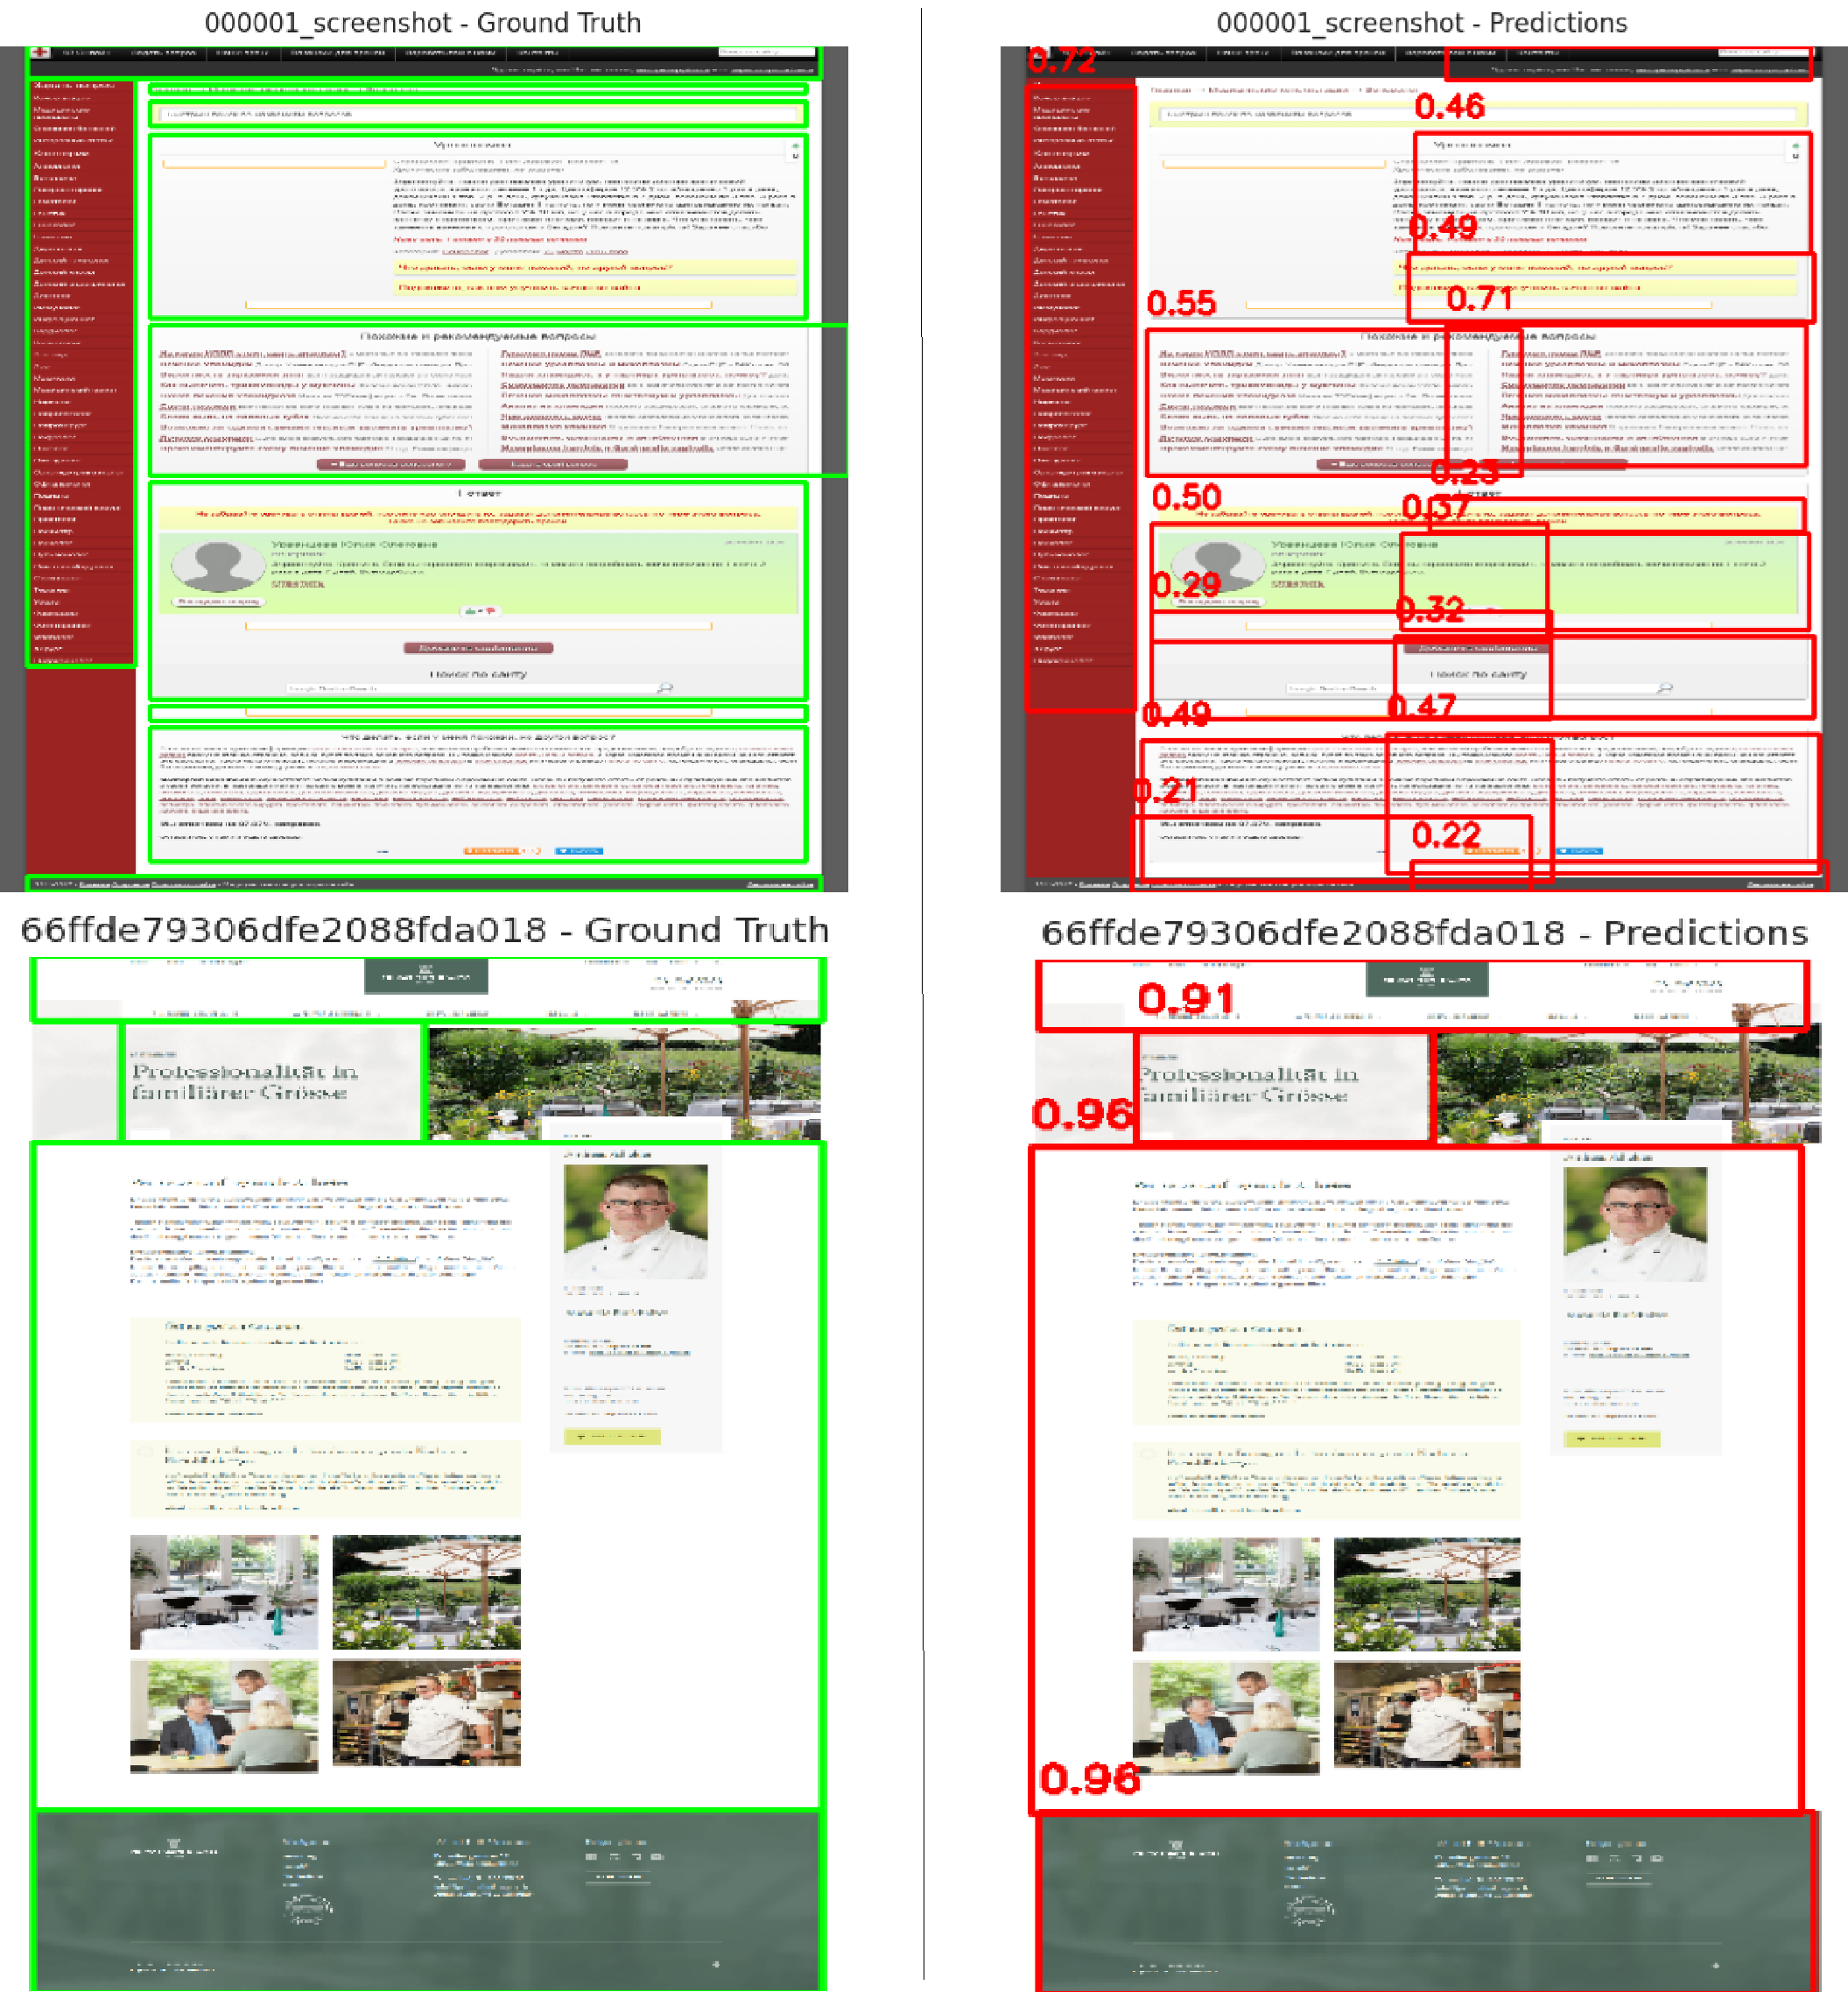
\includegraphics[width=0.8\columnwidth]{label_vs_prediction.png}}
\caption{Comparison of ground truth labels (left) and model predictions (right) on Webis-Webseg-20 dataset (top) and Nano (bottom). Predictions were generated using the standard YOLOv5s model trained on each respective dataset.}
\label{fig:labels}
\end{figure}

Tables~\ref{tab:webis} and~\ref{tab:nano} present performance metrics for various YOLO models using the two post-processing methods NMS (default for YOLO) and WBF. For both methods, we used an IoU threshold of 0.5, with WBF using a skip box threshold of 0.2 and NMS using a confidence threshold of 0.2.

On the Webis-Webseg-20 dataset (Table~\ref{tab:webis}), our implementation results fall significantly below the original paper's reported performance. While our YOLO-WS implementation achieves the highest precision (0.75) with WBF post-processing, its low recall (0.16) suggests unsuccessful training. The standard YOLOv5s implementation also fails to replicate the baseline performance reported in the original YOLO-WS paper. YOLOv11s shows slight improvements over YOLOv5s, achieving the best F1-score (0.48) with standard NMS processing. Notably, during YOLOv5s training, the AutoAnchor system reported poor anchor fit with a low best possible recall (0.588 for 512x512 pixel input, 0.667 for 1024x1024 pixel rectangular input), and critically, a high number of labels found to be less than 3 pixels in size (28,100 of 110,311 labels for 512x512 pixel input, 14710 of 110311 for 1024x1024 pixel rectangular input). The WBF post-processing method consistently improved precision at the cost of recall across all models.

In contrast, our experiments on the Nano dataset (Table~\ref{tab:nano}) achieved substantially better results with just 80 training images. Standard YOLOv5s performed nearly as well as YOLOv11s, while our YOLO-WS implementation continued to show poor performance. YOLOv11s achieved the best overall performance with an F1-score (macro) of 0.89 using rectangular input images, though the improvement from 512x512 pixel images was marginal. Interestingly, increasing input size showed no performance improvement on Webis-Webseg-20. Setting the input size to the YOLO standard (640px) only improved performance of YOLOv5s performance but not YOLOv11s.

\section{Related Work}
The field of web segmentation has explored diverse approaches, ranging from DOM-based methods to purely visual techniques, alongside the development of numerous datasets. Early datasets like News600 Corpus \cite{spengler} and WEBKB Dataset \cite{pasupathi} prioritized specific content types and DOM annotations. The Webis-Webseg-20 dataset \cite{kiesel:2020b} significantly advanced visual evaluation by providing a large-scale, visually annotated benchmark. In subsequent work, the Webis-Webseg-20 authors and others tested various visual-only models \cite{kiesel:2021a, cormer, chen2019mmdetection}, finding their performance comparable to traditional methods, most notably the classical VIPS algorithm \cite{VIPS}.  However, a consistent challenge across these methods, including the visual models and VIPS, is their limited generalization to diverse and complex web page layouts. Indeed, even recent approaches like YOLO-WS fail to significantly surpass the performance of classical techniques like VIPS, highlighting the need for further innovation in robust web page segmentation.

\section{Discussion \& Future Research}
In this paper, we re-implemented YOLO-WS, a purely visual-based web segmentation algorithm. Our experiments on the datasets Webis-Webseg-20 and Nano reveal that achieving high performance in visual web segmentation might be more accessible than previously suggested. While our reimplementation did not reach the performance levels reported in the original paper, standard YOLOv5s and especially the successor YOLOv11s demonstrated surprising results on our Nano dataset with only 80 images for training. This suggests that purely visual approaches are effective for web segmentation. 

The contrast between Nano and Webis-Webseg-20 results shows the importance of high-quality data. As shown in Fig.~\ref{fig:bounding_boxes} and Fig.~\ref{fig:width_height_ratio}, the Webis-Webseg-20 dataset exhibits not only a significantly smaller bounding box area distribution (Nano average: 40'716.17 pixels$^2$, minimum area 594.95 pixels$^2$ vs. Webis-Webseg-20 average: 9'628.91 pixels$^2$, minimum area: 0.01 pixels$^2$) but the website screenshots tend to be much taller and narrower compared to the Nano dataset. This could explain the difficulties encountered in training models effectively on Webis-Webseg-20.

\begin{figure}[htbp]
\centerline{\includegraphics[width=0.6\columnwidth, height=3.65in]{bounding_box_area.png}}
\caption{Nano (top) vs. Webis-Webseg-20 (bottom) Bounding Box Area Distributions.}
\label{fig:bounding_boxes}
\end{figure}

\begin{figure}[htbp]
\centerline{\includegraphics[width=0.65\columnwidth, height=2.9in]{width_height_ratio.png}}
\caption{Nano (top) vs. Webis-Webseg-20 (bottom) Aspect Ratio Distributions.}
\label{fig:width_height_ratio} 
\end{figure}

\subsection{Future Research}

Our success with the Nano dataset using only 80 training images raises an important question about the minimum amount of high-quality data needed for effective YOLO-based web segmentation. A systematic study of varying training set sizes with high-quality annotations could establish practical guidelines for dataset creation and model training. Future research should also compare purely visual models and mixed models (visual + DOM) to clearly delineate their respective strengths and use cases. Finally, while we focused on the YOLO family, research needs to extend to other architectures and make a comparison to antecedent classical models.

\begin{thebibliography}{00}
\bibitem{VIPS} Cai, Deng \& Yu, Shipeng \& Wen, Ji-Rong \& Ma, Wei-Ying. (2003). VIPS: a Vision-based Page Segmentation Algorithm. 
\bibitem{DOM-structure} Huynh, Hieu \& Nguyen, Vu \& Nguyen, Tien. (2024). A DOM-structural Cohesion Analysis Approach for Segmentation of Modern Web Pages. 10.21203/rs.3.rs-4392630/v1. 
\bibitem{HEPS} Tomohiro Manabe and Keishi Tajima. 2015. Extracting logical hierarchical structure of HTML documents based on headings. Proc. VLDB Endow. 8, 12 (August 2015), 1606–1617. https://doi.org/10.14778/2824032.2824058
\bibitem{kiesel:2020b} Kiesel, Johannes and Kneist, Florian and Meyer, Lars and Komlossy, Kristof and Stein, Benno and Potthast, Martin. (2020). Web Page Segmentation Revisited: Evaluation Framework and Dataset. In *29th ACM International Conference on Information and Knowledge Management (CIKM 2020)*, 3047--3054. ACM. https://doi.org/10.1145/3340531.3412782
\bibitem{yolov5} Ultralytics. (2021). YOLOv5: A state-of-the-art real-time object detection system. https://docs.ultralytics.com 
\bibitem{cormer} Cormer, Michael \& Mann, Richard \& Moffatt, Karyn \& Cohen, Robin. (2017). Towards an Improved Vision-Based Web Page Segmentation Algorithm. 345-352. 10.1109/CRV.2017.38.
\bibitem{coordatt} Hou, Qibin, Daquan Zhou and Jiashi Feng. “Coordinate Attention for Efficient Mobile Network Design.” 2021 IEEE/CVF Conference on Computer Vision and Pattern Recognition (CVPR) (2021): 13708-13717.
\bibitem{frelu} Ningning Ma, Xiangyu Zhang, and Jian Sun. 2020. Funnel Activation for Visual Recognition. In Computer Vision – ECCV 2020: 16th European Conference, Glasgow, UK, August 23–28, 2020, Proceedings, Part XI. Springer-Verlag, Berlin, Heidelberg, 351–368. https://doi.org/10.1007/978-3-030-58621-8\_21 %%%
\bibitem{YOLO-WS} Li Dai, Zunwang Ke, and Wushour Silamu. 2023. YOLO-WS: A Novel Method for Webpage Segmentation. In Proceedings of the 2023 4th International Conference on Computing, Networks and Internet of Things (CNIOT '23). Association for Computing Machinery, New York, NY, USA, 451–456. https://doi.org/10.1145/3603781.3603862
\bibitem{huynh_web_2023} Huynh, Minh-Hieu \& Le, Quoc-Tri \& Nguyen, Vu \& Nguyen, Tien. (2023). Web Page Segmentation: A DOM-Structural Cohesion Analysis Approach. In *Web Information Systems Engineering – WISE 2023*, 319–333. https://doi.org/10.1007/978-981-99-7254-8\_25
\bibitem{spengler} Spengler, Alex \& Gallinari, Patrick. (2010). Document structure meets page layout: loopy random fields for web news content extraction. In Proceedings of the 10th ACM symposium on Document engineering, 151-160. https://doi.org/10.1145/1860559.1860590
\bibitem{pasupathi} Pasupathi. (2012). Web Document Segmentation Using Frequent Term Sets For Summarization. Journal of Computer Science, 8(12), 2053-2061. https://doi.org/10.3844/jcssp.2012.2053.2061
\bibitem{feiou} Yi-Fan Zhang, Weiqiang Ren, Zhang Zhang, Zhen Jia, Liang Wang, and Tieniu Tan. 2022. Focal and efficient IOU loss for accurate bounding box regression. Neurocomput. 506, C (Sep 2022), 146–157. https://doi.org/10.1016/j.neucom.2022.07.042
\bibitem{wbf} Solovyev, Roman and Wang, Weimin and Gabruseva, Tatiana. (2021). Weighted boxes fusion: Ensembling boxes from different object detection models. Image and Vision Computing, 107, 104117. http://dx.doi.org/10.1016/j.imavis.2021.104117
\bibitem{kiesel:2021a} Kiesel, Johannes, Lars Meyer, Florian Kneist, Benno Stein and Martin Potthast. 2021. “An Empirical Comparison of Web Page Segmentation Algorithms.” In Advances in Information Retrieval. 43rd European Conference on IR Research (ECIR 2021), 62–74. Springer, Berlin Heidelberg New York. https://doi.org/10.1007/978-3-030-72240-1\_5
\bibitem{chen2019mmdetection} Chen, Kai, Jiaqi Wang, Jiangmiao Pang, Yuhang Cao, Yu Xiong, Xiaoxiao Li, Shuyang Sun, et al. 2019. “MMDetection: Open MMLab Detection Toolbox and Benchmark.” arXiv:1906.07155 [cs.CV]. https://arxiv.org/abs/1906.07155
\end{thebibliography}
%TODO: use numbers for reference
%TODO: add iteration per second per model

%\section{Prepare Your Paper Before Styling}
%Before you begin to format your paper, first write and save the content as a 
%separate text file. Complete all content and organizational editing before 
%formatting. Please note sections \ref{AA} to \ref{FAT} below for more information on 
%proofreading, spelling and grammar.

%Keep your text and graphic files separate until after the text has been 
%formatted and styled. Do not number text heads---{\LaTeX} will do that 
%for you.

%\subsection{Abbreviations and Acronyms}\label{AA}
%Define abbreviations and acronyms the first time they are used in the text, 
%even after they have been defined in the abstract. Abbreviations such as 
%IEEE, SI, MKS, CGS, ac, dc, and rms do not have to be defined. Do not use 
%abbreviations in the title or heads unless they are unavoidable.

%\subsection{Units}
%\begin{itemize}
%\item Use either SI (MKS) or CGS as primary units. (SI units are encouraged.) English units may be used as secondary units (in parentheses). An exception would be the use of English units as identifiers in trade, such as ``3.5-inch disk drive''.
%\item Avoid combining SI and CGS units, such as current in amperes and magnetic field in oersteds. This often leads to confusion because equations do not balance dimensionally. If you must use mixed units, clearly state the units for each quantity that you use in an equation.
%\item Do not mix complete spellings and abbreviations of units: ``Wb/m\textsuperscript{2}'' or ``webers per square meter'', not ``webers/m\textsuperscript{2}''. Spell out units when they appear in text: ``. . . a few henries'', not ``. . . a few H''.
%\item Use a zero before decimal points: ``0.25'', not ``.25''. Use ``cm\textsuperscript{3}'', not ``cc''.)
%\end{itemize}

%\subsection{Equations}
%Number equations consecutively. To make your 
%equations more compact, you may use the solidus (~/~), the exp function, or 
%appropriate exponents. Italicize Roman symbols for quantities and variables, 
%but not Greek symbols. Use a long dash rather than a hyphen for a minus 
%sign. Punctuate equations with commas or periods when they are part of a 
%sentence, as in:
%\begin{equation}
%a+b=\gamma\label{eq}
%\end{equation}

%Be sure that the 
%symbols in your equation have been defined before or immediately following 
%the equation. Use ``\eqref{eq}'', not ``Eq.~\eqref{eq}'' or ``equation \eqref{eq}'', except at 
%the beginning of a sentence: ``Equation \eqref{eq} is . . .''

%\subsection{\LaTeX-Specific Advice}

%Please use ``soft'' (e.g., \verb|\eqref{Eq}|) cross references instead
%of ``hard'' references (e.g., \verb|(1)|). That will make it possible
%to combine sections, add equations, or change the order of figures or
%citations without having to go through the file line by line.

%Please don't use the \verb|{eqnarray}| equation environment. Use
%\verb|{align}| or \verb|{IEEEeqnarray}| instead. The \verb|{eqnarray}|
%environment leaves unsightly spaces around relation symbols.

%Please note that the \verb|{subequations}| environment in {\LaTeX}
%will increment the main equation counter even when there are no
%equation numbers displayed. If you forget that, you might write an
%article in which the equation numbers skip from (17) to (20), causing
%the copy editors to wonder if you've discovered a new method of
%counting.

%{\BibTeX} does not work by magic. It doesn't get the bibliographic
%data from thin air but from .bib files. If you use {\BibTeX} to produce a
%bibliography you must send the .bib files. 

%{\LaTeX} can't read your mind. If you assign the same label to a
%subsubsection and a table, you might find that Table I has been cross
%referenced as Table IV-B3. 

%{\LaTeX} does not have precognitive abilities. If you put a
%\verb|\label| command before the command that updates the counter it's
%supposed to be using, the label will pick up the last counter to be
%cross referenced instead. In particular, a \verb|\label| command
%should not go before the caption of a figure or a table.

%Do not use \verb|\nonumber| inside the \verb|{array}| environment. It
%will not stop equation numbers inside \verb|{array}| (there won't be
%any anyway) and it might stop a wanted equation number in the
%surrounding equation.

%\subsection{Some Common Mistakes}\label{SCM}
%\begin{itemize}
%\item The word ``data'' is plural, not singular.
%\item The subscript for the permeability of vacuum $\mu_{0}$, and other common scientific constants, is zero with subscript formatting, not a lowercase letter ``o''.
%\item In American English, commas, semicolons, periods, question and exclamation marks are located within quotation marks only when a complete thought or name is cited, such as a title or full quotation. When quotation marks are used, instead of a bold or italic typeface, to highlight a word or phrase, punctuation should appear outside of the quotation marks. A parenthetical phrase or statement at the end of a sentence is punctuated outside of the closing parenthesis (like this). (A parenthetical sentence is punctuated within the parentheses.)
%\item A graph within a graph is an ``inset'', not an ``insert''. The word alternatively is preferred to the word ``alternately'' (unless you really mean something that alternates).
%\item Do not use the word ``essentially'' to mean ``approximately'' or ``effectively''.
%\item In your paper title, if the words ``that uses'' can accurately replace the word ``using'', capitalize the ``u''; if not, keep using lower-cased.
%\item Be aware of the different meanings of the homophones ``affect'' and ``effect'', ``complement'' and ``compliment'', ``discreet'' and ``discrete'', ``principal'' and ``principle''.
%\item Do not confuse ``imply'' and ``infer''.
%\item The prefix ``non'' is not a word; it should be joined to the word it modifies, usually without a hyphen.
%\item There is no period after the ``et'' in the Latin abbreviation ``et al.''.
%\item The abbreviation ``i.e.'' means ``that is'', and the abbreviation ``e.g.'' means ``for example''.
%\end{itemize}
%An excellent style manual for science writers is \cite{b7}.

%\subsection{Authors and Affiliations}\label{AAA}
%\textbf{The class file is designed for, but not limited to, six authors.} A 
%minimum of one author is required for all conference articles. Author names 
%should be listed starting from left to right and then moving down to the 
%next line. This is the author sequence that will be used in future citations 
%and by indexing services. Names should not be listed in columns nor group by 
%affiliation. Please keep your affiliations as succinct as possible (for 
%example, do not differentiate among departments of the same organization).

%\subsection{Identify the Headings}\label{ITH}
%Headings, or heads, are organizational devices that guide the reader through 
%your paper. There are two types: component heads and text heads.

%Component heads identify the different components of your paper and are not 
%topically subordinate to each other. Examples include Acknowledgments and 
%References and, for these, the correct style to use is ``Heading 5''. Use 
%``figure caption'' for your Figure captions, and ``table head'' for your 
%table title. Run-in heads, such as ``Abstract'', will require you to apply a 
%style (in this case, italic) in addition to the style provided by the drop 
%down menu to differentiate the head from the text.

%Text heads organize the topics on a relational, hierarchical basis. For 
%example, the paper title is the primary text head because all subsequent 
%material relates and elaborates on this one topic. If there are two or more 
%sub-topics, the next level head (uppercase Roman numerals) should be used 
%and, conversely, if there are not at least two sub-topics, then no subheads 
%should be introduced.

%\subsection{Figures and Tables}\label{FAT}
%\paragraph{Positioning Figures and Tables} Place figures and tables at the top and 
%bottom of columns. Avoid placing them in the middle of columns. Large 
%figures and tables may span across both columns. Figure captions should be 
%below the figures; table heads should appear above the tables. Insert 
%figures and tables after they are cited in the text. Use the abbreviation 
%``Fig.~\ref{fig}'', even at the beginning of a sentence.

%\begin{table}[htbp]
%\caption{Table Type Styles}
%\begin{center}
%\begin{tabular}{|c|c|c|c|}
%\hline
%\textbf{Table}&\multicolumn{3}{|c|}{\textbf{Table Column Head}} \\
%\cline{2-4} 
%\textbf{Head} & \textbf{\textit{Table column subhead}}& \textbf{\textit{Subhead}}& \textbf{\textit{Subhead}} \\
%\hline
%copy& More table copy$^{\mathrm{a}}$& &  \\
%\hline
%\multicolumn{4}{l}{$^{\mathrm{a}}$Sample of a Table footnote.}
%\end{tabular}
%\label{tab1}
%\end{center}
%\end{table}
%\begin{figure}[htbp]
%\centerline{\includegraphics{fig1.png}}
%\caption{Example of a figure caption.}
%\label{fig}
%\end{figure}

%Figure Labels: Use 8 point Times New Roman for Figure labels. Use words 
%rather than symbols or abbreviations when writing Figure axis labels to 
%avoid confusing the reader. As an example, write the quantity 
%``Magnetization'', or ``Magnetization, M'', not just ``M''. If including 
%units in the label, present them within parentheses. Do not label axes only 
%with units. In the example, write ``Magnetization (A/m)'' or ``Magnetization 
%\{A[m(1)]\}'', not just ``A/m''. Do not label axes with a ratio of 
%quantities and units. For example, write ``Temperature (K)'', not 
%``Temperature/K''.

%\section*{References}

%Please number citations consecutively within brackets \cite{b1}. The 
%sentence punctuation follows the bracket \cite{b2}. Refer simply to the reference 
%number, as in \cite{b3}---do not use ``Ref. \cite{b3}'' or ``reference \cite{b3}'' except at 
%the beginning of a sentence: ``Reference \cite{b3} was the first $\ldots$''

%Number footnotes separately in superscripts. Place the actual footnote at 
%the bottom of the column in which it was cited. Do not put footnotes in the 
%abstract or reference list. Use letters for table footnotes.

%Unless there are six authors or more give all authors' names; do not use 
%``et al.''. Papers that have not been published, even if they have been 
%submitted for publication, should be cited as ``unpublished'' \cite{b4}. Papers 
%that have been accepted for publication should be cited as ``in press'' \cite{b5}. 
%Capitalize only the first word in a paper title, except for proper nouns and 
%element symbols.

%For papers published in translation journals, please give the English 
%citation first, followed by the original foreign-language citation \cite{b6}.

%\vspace{12pt}
%\color{red}
%IEEE conference templates contain guidance text for composing and formatting conference papers. Please ensure that all template text is removed from your conference paper prior to submission to %the conference. Failure to remove the template text from your paper may result in your paper not being published.

\end{document}

